\documentclass[conference]{IEEEtran}
\usepackage{cite}
\usepackage{amsmath}
\usepackage{graphicx}
\usepackage{booktabs}
\usepackage{url}
\usepackage{hyperref}
\graphicspath{{../figures/}}
\hypersetup{colorlinks=true, urlcolor=blue, citecolor=blue, linkcolor=black}

\title{Flagging Missed Clinic Appointments from the Booking Screen: Linear Models, Forests, and a Small Neural Net}

\author{%
\IEEEauthorblockN{Sammy Niyonkuru}
}

\begin{document}
\maketitle

\noindent\textit{Code repository:} [insert the public GitHub URL for this project]\\
\textit{Google Drive folder} (zipped raw dataset, \texttt{.joblib} weights, and Keras \texttt{.h5} / \texttt{.keras} weights; anyone with the link can view): [insert the Drive folder URL]\\
\textit{Video recording} (problem, data, method, experiments, and what I would not deploy): [insert the video URL]

\begin{abstract}
Missed appointments leave a slot empty and make the queue longer for the people who do come. I treat that as a classification problem decided at the moment a visit is booked, which is the moment a clerk could still send a reminder or avoid stacking the same clinician with several fragile bookings. The data are the public Medical Appointment No Shows extract: 110,527 appointments, of which 110,514 remain after I drop impossible ages and five negative waits. About 20.2\% are no-shows. I compare logistic regression, a linear SVM, random forests, histogram gradient boosting, and five neural networks trained with \texttt{tf.data}. Patients are not shared across train, validation, and test. On the test patients a depth-limited forest reaches ROC-AUC 0.736 and a small multilayer perceptron reaches 0.731. A logistic model with no personal history already reaches 0.716, and the raw lead time alone reaches 0.693. The forest is real, and it is a small step past ``flag the booking if it is not for today.'' I would use the score to order reminder calls. I would not cancel a slot with it, and I would not ship these weights to a clinic in Nigeria or South Africa without a local file. The extract covers six weeks in Vit\'{o}ria, Brazil, and it does not contain transport cost, distance, or the reason for the last miss.
\end{abstract}

\section{Introduction}
My aim with this project is practical. I want booking in busy clinics, including public facilities in African cities, to be a record the desk can act on, rather than a paper list that is already wrong by mid-morning. Overcrowding and long waits are not only a matter of too few clinicians. They are also a matter of slots that were held for someone who never arrived, and of sessions that then run late for everyone else. Levesque, Harris, and Russell describe access as the fit between the patient and the service, not as a gate that is either open or shut \cite{levesque2013}. A booking that is made and then missed is a failure of that fit. The person may have had no money for the trip, may have forgotten, or may have been given a date so far away that the original complaint changed. The clinic experiences all of those as an empty chair.

Dantas and colleagues, reviewing 105 studies, put the average no-show rate near 23\%, and the African studies in that review near 43\% \cite{dantas2018}. That comparison is why this is the classification problem I chose. Facility-level work in Nigeria and South Africa, which I discuss in Section~\ref{sec:lit}, finds the same operational mess and adds a clinical one: at an HIV clinic in Johannesburg, repeated early misses predicted death and leaving care \cite{brennan2010}. A score that only fills slots can work against the reason the visit existed.

The decision I model is binary and early. At the time the clerk confirms the booking, will this visit be missed? A useful score would change the order of reminder calls, or tell a supervisor which sessions are carrying several high-risk bookings. It would not, by itself, be a reason to give the slot to someone else. False alarms are not free. If the clinic overbooks every flagged visit, the people who were going to attend wait longer, which is the harm I am trying to reduce.

Two modelling habits in this literature make the headline number hard to trust. The first is accuracy. When four in five people attend, a classifier that never predicts a miss is about 80\% accurate and operationally empty. Carreras-Garc\'{i}a and colleagues found that almost none of the fifty prediction papers they reviewed beat the show rate on accuracy, and only one reported an area under the ROC curve above 0.9 \cite{carreras2020}. The second habit is splitting appointments as if they were independent people. The same patient then sits in the training set and the test set, and any feature that remembers their past behaviour looks more powerful than it will be for a new patient. I split by patient. I also refuse to count a visit as ``history'' unless it had already happened on a day before the booking was made. Both choices are easy to get wrong, and the second one is easy to miss because the appointment timestamp in this file is stored at midnight.

\section{Literature Review}
\label{sec:lit}
\subsection{What the operations papers agree on}
Dantas et al.\ find a long lead time and a previous miss across specialties, with younger age, lower socioeconomic position, and distance close behind \cite{dantas2018}. Kheirkhah et al.\ count the empty clinician time that follows \cite{kheirkhah2016}. The African papers are small surveys, weak for prediction and useful for causes. At Bida, 44\% of 315 outpatients had missed a visit, mostly from forgetting, treatment cost, transport cost, or work, and more often if they lived outside town \cite{omokanye2021}. Calabar psychiatry was lower at 16.6\%, with the same three reasons \cite{edet2024}. At Baragwanath audiology just over half of adults did not return; a reminder helped, and so did understanding why the visit mattered, which is not the same thing \cite{khan2023}. Brennan et al.\ change the objective: at Themba Lethu, repeated early misses on antiretroviral therapy predicted death and leaving care \cite{brennan2010}. My file has no diagnosis, so I cannot optimise for that, and I should not pretend attendance is the whole goal.

\subsection{What the prediction papers actually achieved}
Carreras-Garc\'{i}a et al.\ reviewed fifty prediction studies. Logistic regression was still the usual tool, and prior no-show rate was the feature most often called decisive. Beating the show rate on accuracy was rare, and a ROC-AUC above 0.9 appeared once \cite{carreras2020}. I read that as a ceiling, not as a dare to stack more layers.

Three papers bound the number I should expect. Lenzi, Ben, and Stein reported a validation AUC of 0.809 on 40,740 primary-care appointments in Porto Alegre (13\% no-shows), with previous attendance and same-day booking doing the work \cite{lenzi2019}. Their file runs from 2011 to 2014, so ``previous attendance'' is a history, not a single earlier row. Mohammadi et al.\ compared logistic regression, a neural net, and naive Bayes on 73,811 community-health-centre appointments; naive Bayes reached about 0.86, and the useful fields were lead time, prior misses, cell-phone ownership, and days since the last visit \cite{mohammadi2018}. The phone result is a warning: an SMS flag is empty if the number on the card is a neighbour's. Nelson et al.\ reached 0.852 with gradient boosting on 22,318 MRI appointments, but they needed on the order of eighty variables, and they argue that low-dimensional linear models are the wrong tool once causes multiply \cite{nelson2019}. I agree, and a public booking desk often has age, sex, the date, and a few chronic-disease ticks. It does not have eighty fields.

So the operations papers say lead time, forgetting, money, and distance, while the prediction papers get high AUCs from long records. I want the AUC of a short booking-time vector, whether a neural net beats a linear model on it, and whether either beats the sentence ``flag it if it is not today.'' Public notebooks on this same file often shuffle appointments and shift the previous label, so the same person trains and tests the model. That AUC does not answer the question about the next patient.

\subsection{Bias, variance, and the metrics that match the decision}
Hastie, Tibshirani, and Friedman separate a model that cannot follow the signal from one that fits noise \cite{hastie2009}. Logistic regression is the rigid end: with a linear log-odds, more rows of the same columns should not move validation AUC much. A random forest averages noisy trees and can still memorise if the leaves are pure \cite{breiman2001}. In Friedman's boosting the learning rate and the depth are the bias--variance knobs \cite{friedman2001}. A multilayer perceptron can represent interactions a line misses \cite{goodfellow2016}, but on a narrow table the extra capacity has to be spent somewhere, which is why dropout is in the deeper nets \cite{srivastava2014}. I train with Adam \cite{kingma2015} and then change only the learning rate, so that comparison is not confounded by a schedule. Saito and Rehmsmeier show that ROC looks kinder than precision--recall when the positive class is uncommon \cite{saito2015}. At a 20\% no-show rate ROC-AUC is still the number the papers above quote, so I report it, and I treat precision at a chosen recall as the number a clerk would feel. A threshold of 0.5 is a default, not a cost ratio. The two errors do not cost the same.

\section{Methodology}
\label{sec:method}
\subsection{Data}
The file is Joni Hoppen's Kaggle extract, CC BY-NC-SA 4.0 \cite{hoppen2016}: 110,527 appointments with sex, booking day, visit day, age, neighbourhood, a Bolsa Fam\'{i}lia flag, hypertension, diabetes, alcoholism, a handicap count, an SMS flag, and the no-show label. The neighbourhoods are districts of Vit\'{o}ria, and the visits run from 29 April to 8 June 2016. I did not find an open African appointment file of this size, so this Brazilian extract is a stand-in. That limit belongs in the paper, not in a footnote.

I read \texttt{PatientId} as a string. The identifier is a large integer, and reading it as a float merges distinct people. The positive class is a no-show, which the file codes as \texttt{Yes}. That coding is easy to invert, so every metric below is for the miss, not for attendance.

Cleaning removed 13 rows. One age was $-1$ and seven ages were above 100, which I do not believe as dates of birth on a booking card. Five rows had an appointment date before the scheduling date. I did not impute these. They are not missing values in the ordinary sense. They are rows I cannot defend. No appointment identifier was duplicated, and sex took only the values F and M. After that filter the table has 110,514 appointments, 62,294 patients, and 22,311 no-shows (20.19\%). There are 81 neighbourhoods.

The lead time is the difference in calendar dates, not in timestamps. The visit time in this file is always midnight. If I subtract the raw timestamps, a booking made at 18:00 for a visit the same calendar day looks like a negative wait. I made that mistake in a first pass and briefly thought several thousand rows were corrupt. They were same-day afternoon bookings. Same-day bookings are 34.9\% of the cleaned file, and their no-show rate is 4.6\%. Bookings for a later day are missed 28.5\% of the time. Any pipeline that drops ``negative lead time'' computed from the raw clock will throw away the most informative group in the table.

\subsection{Features that exist at booking time}
The main models see the booking screen plus visits that had already happened: age, lead time and its log, a same-day flag, sex, scholarship, the three conditions and their count, handicap, booking hour, and weekday as a sine and cosine. I drop month. Six weeks cannot support one.

History is computed per patient. A past visit counts only when its appointment date is strictly earlier than the date the current visit was booked. Visits on the booking day itself do not count, because I cannot tell from a date-only stamp whether they had already happened. I checked this on a hand-built patient with four bookings. A visit booked on 1 May for 10 June does not inherit the outcome of a visit that occurs on 20 May, even though 20 May is before 10 June, because on 1 May that later visit had not happened and in this example had not even been booked. The unit test for that case is in the repository. A naive shift along the appointment date would have leaked it.

Only 27.9\% of rows have any such prior visit. That is a direct consequence of the six-week window. The mean prior no-show rate is 0.053 among people who attend and 0.065 among people who miss. The separation is real and small. Neighbourhood is stored two ways for the tabular models: the share of training rows in that neighbourhood, and a smoothed no-show rate, $(s + 30\bar{y})/(n+30)$, with the training rows' own labels kept out of their feature by five-fold out-of-fold encoding. Validation and test use the rate fit on all training rows. Unseen neighbourhoods fall back to the training base rate. The embedding network does not receive those two rates. It receives a neighbourhood index and has to learn the district from the attendance labels.

I left SMS out of the main feature set. Sending a text is an action, not a trait, and in this file it is perfectly tied to lead time: no same-day booking received an SMS. Putting it in the main model would invite someone to read a coefficient as the effect of a reminder. I add it back in one pre-specified logistic ablation.

\subsection{Split}
Appointments from the same patient stay in one split. Within each patient type (never missed, missed at least half of their visits, or somewhere in between) I assign patients so that each split receives about the same share of rows. The result is 75,140 training appointments (42,304 patients), 13,269 validation appointments (7,492 patients), and 22,105 test appointments (12,498 patients). The no-show rates are 20.16\%, 20.30\%, and 20.21\%. The share of rows with a prior visit is also within about one point across the three splits.

The first version of this splitter did not do that. It filled the test set by walking patient types in turn. The types who sometimes miss were used up in the test and validation sets, and the training set was left with people who always attend. On a smoke-test sample the training no-show rate fell to about 14\% while validation and test sat near 30\%. Every comparison after that would have been a comparison of different populations. I rewrote the split before the full run. I report this because it changed the experiment, and because it is the sort of bug a row-count check does not catch if you only look at the 80/20 ratio.

Hyperparameters that I search over are chosen on an inner patient holdout carved from the training patients (25\% of those rows), or, for the networks, by early stopping on the validation patients. The test patients are scored after that choice. The threshold that maximises the no-show F1 is also chosen on validation scores and then frozen. I do not retune it on the test set.

One comparison breaks the patient rule on purpose. Experiment E10 refits the class-weighted logistic model on a stratified random split of appointments. In that split, 9,714 patients appear on both sides. I wanted the size of the optimism, not a second leaderboard entry.

\subsection{Models and the runs}
Traditional models are scikit-learn estimators. The networks are Keras models, Sequential for E11--E14 and Functional for E15, trained from a shuffled \texttt{tf.data} pipeline at batch size 512. One seed fixes the split and the forests.

E00 scores every row with the training prevalence, so a threshold of 0.5 means ``everyone attends.'' E01 is unweighted logistic regression without history ($C=1$); E02 adds history; E03 adds balanced class weights. A grid $C \in \{0.01, 0.1, 1, 10\}$ on the inner holdout was flat (inner AUC 0.7269 down to 0.7268), and I kept $C=0.01$. E04 is a forest of 200 trees, depth 12, minimum leaf 5, with \texttt{balanced\_subsample} weights. E05 searches depth $\{8, 12, 16, \text{unlimited}\}$, leaf $\{2, 5, 10\}$, and feature fraction sqrt or 0.5, at 120 trees, then refits the winner with 260. E06 is histogram gradient boosting, learning rate 0.08, depth 6, $\ell_2=1$, early stopping. E07 raises the learning rate to 0.2 and cuts depth to 3. E08 is a linear SVM; the alert rule uses the sign of the margin. E09 adds SMS to E03. E10 is the random row split.

E11 has dense layers 64 and 32, dropout 0.2, class weights, Adam at $10^{-3}$. E12 uses 128, 64, and 32 with batch normalisation and dropout 0.35. E13 keeps that net and sets the learning rate to $10^{-2}$, with no schedule, so the only change from E12 is the step size. E14 drops the class weights. E15 embeds neighbourhood (dimension 8) and concatenates it with the numeric inputs before dense layers of 64 and 32. Early stopping monitors validation ROC-AUC, patience 5, and restores the best weights.

I did not use SMOTE. The minority class is 20\%, not 1\%, and synthetic patients would have blurred the line the brief draws against generated data. Class weights and a moved threshold were enough to show the imbalance. I also did not tune a cost matrix. I do not know the local cost of a wasted slot relative to a false reminder, and inventing one would have produced a sharp threshold with a made-up justification.

The saved traditional model is the one with the highest validation ROC-AUC among E02--E08. The saved network is the one with the highest validation ROC-AUC among E11--E15, except that I keep E11 when it is within 0.002 of that best validation AUC. A rerun once handed the save to E13 because the third decimal moved, and I am not going to change the architecture over that. Test AUC did not vote. Every run is written to \texttt{experiments/runs/}, to a results table, to TensorBoard event files for the networks, and to a Weights \& Biases log in offline mode.

\section{Results}
\label{sec:results}
\subsection{What the cohort looks like before any model}
Fig.~\ref{fig:lead} is the result I would show a clinic manager before any ROC curve. Same-day bookings are missed 4.6\% of the time ($n=38{,}560$). The rate is 22.7\% at one to two days, 24.9\% at three to seven, 30.5\% at eight to fourteen, 32.6\% at fifteen to thirty, and 33.0\% after that. The curve rises quickly and then flattens. Mean lead time is 8.8 days for attenders and 15.8 days for no-shows. Age runs the other way, mildly: younger adults miss more often than older adults, and sex barely differs (20.3\% of women, 20.0\% of men, with women 65\% of the rows). Scholarship holders are 9.8\% of rows and miss 23.7\% of visits, against 19.8\% for everyone else. That is the direction the socioeconomic literature predicts, and it is a Bolsa Fam\'{i}lia flag, not a measure of poverty I would recognise in a Nigerian or Kenyan record.

\begin{figure}[t]
\centering
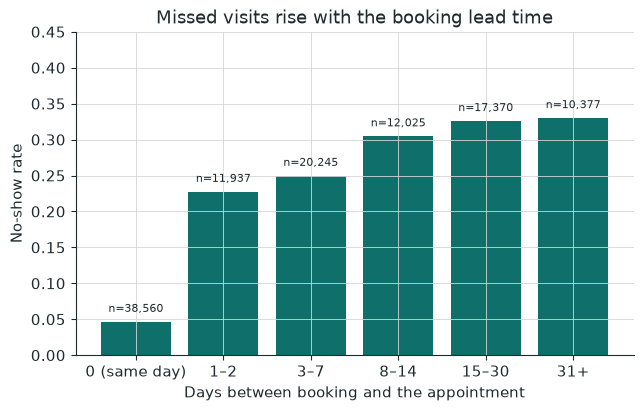
\includegraphics[width=\columnwidth]{eda_lead_time.png}
\caption{No-show rate by lead time on the cleaned cohort of 110,514 appointments. Same-day visits dominate the file and are rarely missed.}
\label{fig:lead}
\end{figure}

The SMS column is a trap if it is read marginally. Bookings that received a text were missed 27.6\% of the time, against 16.7\% for bookings that did not. That looks like a harmful reminder. Fig.~\ref{fig:sms} is the same rate inside lead-time bands. No same-day booking was texted. Inside every band where texts exist, the texted bookings have the lower miss rate, by a few points up to about seven points at the long waits. Among bookings made three or more days ahead, the rates are 27.6\% with an SMS and 32.7\% without. I do not call that a treatment effect. Nobody randomised the text. It is enough to stop me using the crude gap as evidence against reminders, which is the reading a first plot invites.

\begin{figure}[t]
\centering
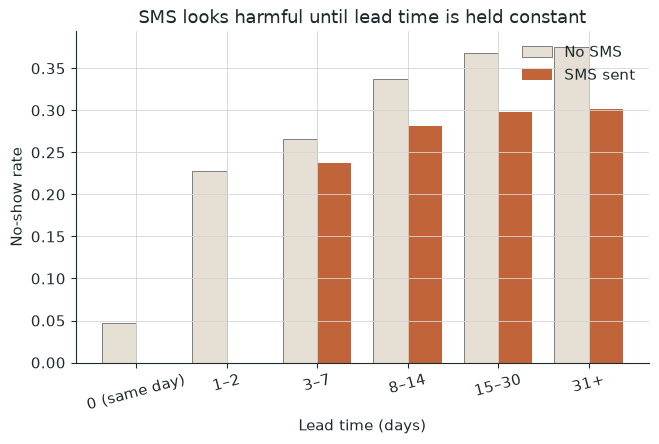
\includegraphics[width=\columnwidth]{eda_sms_by_lead.png}
\caption{No-show rate by lead time and SMS. The crude SMS gap reverses once same-day bookings, which were never texted, are separated out.}
\label{fig:sms}
\end{figure}

\subsection{Held-out performance}
Table~\ref{tab:main} gives the test metrics after the validation threshold was frozen. The majority rule that predicts attendance for everyone has accuracy 79.8\% on the test patients, no-show recall 0, and ROC-AUC 0.5. I do not put that accuracy in the table as a target. It is the number a model has to beat before accuracy means anything, and none of mine do. The forest's accuracy at its F1 threshold is 65.0\%. That is worse than predicting that everyone attends, and it is the expected price of calling some misses correctly.

\begin{table*}[t]
\centering
\caption{Test metrics. Precision, recall, and F1 are for the no-show class at the validation-chosen threshold. AUC does not use that threshold. E10 uses a different split and is not comparable as a deployable score.}
\label{tab:main}
\footnotesize
\begin{tabular}{llcccccc}
\toprule
ID & Model & Val AUC & Test AUC & PR-AUC & Precision & Recall & F1 \\
\midrule
E01 & Logistic, no history & 0.715 & 0.716 & 0.337 & 0.310 & 0.763 & 0.441 \\
E02 & Logistic, full, unweighted & 0.719 & 0.724 & 0.353 & 0.295 & 0.872 & 0.441 \\
E03 & Logistic, balanced, $C{=}0.01$ & 0.719 & 0.724 & 0.352 & 0.296 & 0.875 & 0.442 \\
E04 & Forest, depth 12, leaf 5 & 0.733 & 0.733 & 0.366 & 0.322 & 0.747 & 0.450 \\
E05 & Forest, depth 16, leaf 10 & 0.735 & 0.736 & 0.369 & 0.330 & 0.712 & 0.451 \\
E06 & Boosting, lr 0.08, depth 6 & 0.732 & 0.735 & 0.373 & 0.326 & 0.731 & 0.451 \\
E07 & Boosting, lr 0.20, depth 3 & 0.729 & 0.735 & 0.370 & 0.337 & 0.684 & 0.451 \\
E08 & Linear SVM & 0.719 & 0.724 & 0.352 & 0.296 & 0.873 & 0.442 \\
E09 & E03 plus SMS flag & 0.721 & 0.727 & 0.357 & 0.314 & 0.784 & 0.448 \\
E10 & E03, random row split & 0.724 & 0.727 & 0.349 & 0.304 & 0.832 & 0.445 \\
E11 & MLP 64--32, class weight & 0.728 & 0.731 & 0.367 & 0.319 & 0.754 & 0.449 \\
E12 & MLP 128--64--32, dropout 0.35 & 0.725 & 0.730 & 0.363 & 0.320 & 0.759 & 0.450 \\
E13 & E12 at learning rate $10^{-2}$ & 0.728 & 0.731 & 0.370 & 0.323 & 0.731 & 0.448 \\
E14 & E12, no class weight & 0.726 & 0.731 & 0.363 & 0.323 & 0.764 & 0.454 \\
E15 & Embedding, Functional API & 0.727 & 0.732 & 0.365 & 0.310 & 0.808 & 0.448 \\
\bottomrule
\end{tabular}
\end{table*}

History adds 0.008 test AUC (0.716 to 0.724). That is the six-week window, not a refutation of Lenzi or Mohammadi: most rows have no earlier visit. Class weights do not change logistic AUC. They change 0.5. Unweighted recall at 0.5 is 0.009, and 0.872 once the threshold moves to 0.19. Weighted recall is already 0.854 at 0.5. Brier score goes from 0.145 to 0.216, worse than predicting the base rate (0.161). Reweighting fixed the cutoff and broke the probabilities.

The linear SVM ties the logistic model at test AUC 0.724. Forests and boosting clear that by about a point. Validation selected E05 (test ROC-AUC 0.736, average precision 0.369, F1 0.451). E06 is within 0.001 on ROC-AUC, has the best average precision (0.373) and a better Brier score (0.143), and overfits less. I saved E05 because validation AUC was the rule. I would ship E06 if the number had to be read as a probability. The networks land in between: E11 wins validation at 0.728 and tests at 0.731; the deeper E12 is worse on validation (0.725); E13 at learning rate $10^{-2}$ does not diverge, stalls near 0.728, and stops at epoch 17 once validation loss rises; E14 without class weights keeps the AUC and improves Brier to 0.144 by moving the threshold to 0.24. E15's test AUC is 0.732 and its validation AUC is slightly worse, so I did not save it. A 0.001 test gap is not a win. E09's SMS flag adds 0.003 AUC once lead time is present. E10, with 9,714 patients on both sides of a row split, reaches 0.727 against E03's 0.724. I expected a larger cheat. History is missing for most rows, so sharing a person does not hand over a biography.

\subsection{The forest search, and the learning curves}
Table~\ref{tab:rf} is the inner holdout for the forest. Depth 16 with a minimum leaf of 2 drove the training AUC to 0.923 and the inner validation AUC down to 0.728. That is the run I would have kept if I had been watching the training score. The leaf size of 10 at the same depth was the best inner validation score, 0.733, with a training AUC of 0.860. Unlimited depth with the same leaf was no better. The search did the thing it is supposed to do: it refused the tree that had memorised the inner training patients.

\begin{table}[t]
\centering
\caption{Random-forest search on the inner patient holdout. Training AUC is on the inner training fold. The chosen row is in bold. Trees during the search: 120. The refit used 260.}
\label{tab:rf}
\footnotesize
\begin{tabular}{lccc}
\toprule
Depth / leaf / features & Train AUC & Inner AUC \\
\midrule
8 / 5 / sqrt & 0.766 & 0.730 \\
12 / 5 / sqrt & 0.828 & 0.731 \\
16 / 2 / sqrt & 0.923 & 0.728 \\
\textbf{16 / 10 / sqrt} & \textbf{0.860} & \textbf{0.733} \\
12 / 5 / 0.5 & 0.853 & 0.729 \\
unlimited / 10 / sqrt & 0.888 & 0.733 \\
\bottomrule
\end{tabular}
\end{table}

Fig.~\ref{fig:lc} is the same gap against sample size. Logistic validation AUC moves from 0.715 to 0.719 between a tenth of the training patients and all of them, with the training curve on top: high bias, and more rows will not fix it. E05's validation AUC rises from 0.718 to 0.735 while training AUC falls from 0.902 to 0.855, leaving a gap near 0.12. The leaf constraint reduced the variance and did not remove it. Neither curve is on the way to the 0.85 Nelson et al.\ report from a much wider record \cite{nelson2019}.

\begin{figure}[t]
\centering
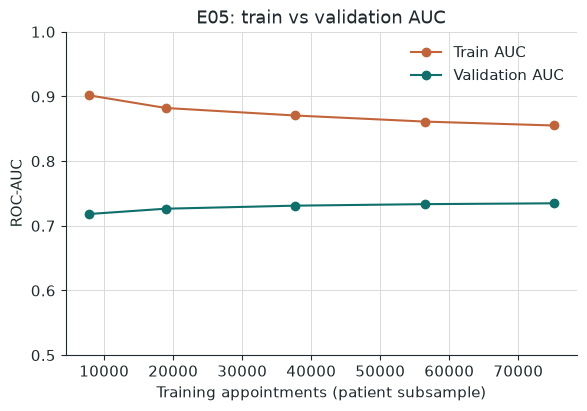
\includegraphics[width=\columnwidth]{learning_curve_tree.png}
\caption{E05 learning curve. Validation AUC inches up. The training curve stays well above it. The logistic curve, not shown at this scale, is flat near 0.72 from the first tenth of the sample.}
\label{fig:lc}
\end{figure}

The network curves tell a related story at a smaller gap. E11's validation AUC moves from 0.720 in the first epoch to about 0.728, and the training AUC ends near 0.742. E12 never catches it. E13 fits faster, is already at validation AUC 0.722 after one epoch, and then sits still while validation loss worsens at the end, which is the early-stopping signal rather than a divergence. I do not have a plot in which a high learning rate explodes. I have a plot in which a high learning rate finishes early and ties the small net. The capacity is not the binding constraint.

\subsection{Errors, and a rule with no model}
On the test set E05's frozen threshold is 0.507. It marks 3,181 true misses, misses 1,286 no-shows, and raises 6,460 false alarms. Precision is 0.330 and recall is 0.712. Of the 9,641 alerts, about two in three are people who will attend. Fig.~\ref{fig:roc} shows why the ROC looks kinder than that sentence. E03, E05, and E11 separate from the diagonal, and they barely separate from each other.

\begin{figure}[t]
\centering
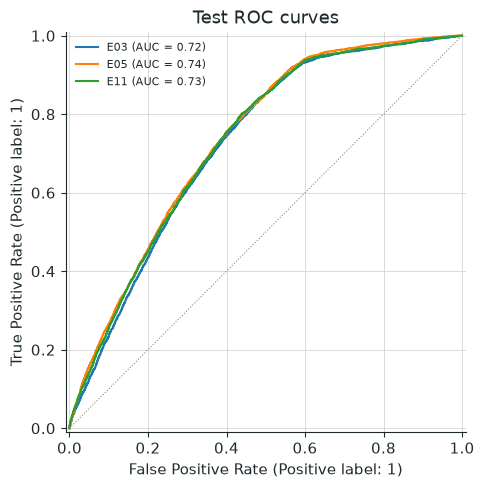
\includegraphics[width=\columnwidth]{roc_test.png}
\caption{Test ROC for the balanced logistic model (E03), the selected forest (E05), and the selected network (E11). The curves sit on top of one another relative to the gap that would change a clinic's policy.}
\label{fig:roc}
\end{figure}

A one-feature score, the lead time itself, has test ROC-AUC 0.693. The rule ``flag if the visit is not today'' has no-show precision 0.282, recall 0.913, and F1 0.430, and it flags 65\% of test bookings. ``Flag if the lead time is three days or more'' has F1 0.431. The forest's F1 is 0.451, at an alert rate of 44\% rather than 55--65\%. The model is the better ranker, and the margin over a sentence a clerk could memorise is thin.

Table~\ref{tab:slice} shows where the forest spends those alerts. Same-day visits (prevalence 5.1\%) are almost left alone: the alert rate is 1.3\%, precision among those few alerts is 0.67, and recall of the rare same-day miss is 0.18. That is a sensible refusal to overbook a group that usually attends. From eight days onward the model alerts on 77\% to 84\% of bookings. Precision stays near one third, because the prevalence itself is only about one third. Past a week, the score is close to ``call them,'' which is the rule the lead-time plot already suggested.

\begin{table}[t]
\centering
\caption{E05 on the test patients, by lead time, at the validation threshold.}
\label{tab:slice}
\footnotesize
\begin{tabular}{lrrrrr}
\toprule
Lead & $n$ & Prevalence & Alert & Precision & Recall \\
\midrule
Same day & 7617 & 0.051 & 0.013 & 0.667 & 0.176 \\
1--2 days & 2381 & 0.213 & 0.412 & 0.273 & 0.528 \\
3--7 & 4108 & 0.254 & 0.505 & 0.307 & 0.612 \\
8--14 & 2394 & 0.299 & 0.774 & 0.322 & 0.831 \\
15--30 & 3450 & 0.322 & 0.841 & 0.343 & 0.894 \\
31+ & 2155 & 0.325 & 0.801 & 0.357 & 0.880 \\
\bottomrule
\end{tabular}
\end{table}

Permutation importance on a validation subsample puts age first (about 0.033 AUC), then log lead time (0.029) and raw lead time (0.025). Same-day adds 0.013 and the prior-no-show rate about 0.003. Sex, handicap, and diabetes are noise. The standardised logistic signs I trust are a large negative on same-day ($-0.79$), a positive on past misses ($+0.22$), and a negative on the count of past visits ($-0.11$). Raw lead time and log lead time have opposite signs because they are the same fact twice; I do not read the negative one as ``waiting helps.''

The cost of leaning on age is in the recall. At the same threshold, no-show recall is 0.89 at ages 18--34 and 0.29 at 65 and over, against prevalences of 23.7\% and 15.7\%. Older patients who will miss are the ones the score skips. Age alone has AUC 0.541, so this is not a one-column sort. It is a sort inside a lead-time band, which is why the permutation and the univariate AUC disagree. If reminders follow the score, that skip is a policy, not a rounding error.

\section{Discussion}
\label{sec:disc}
Another architecture on these columns is not the next experiment. Linear models sit at test AUC 0.724, trees and boosting at 0.734--0.736, networks at 0.730--0.732. The same-day cliff is a threshold a forest can cut and a line only approximates. There is no rich interaction for a deep net, which matches Mohammadi et al., whose neural net did not dominate simpler models \cite{mohammadi2018}, and it is the opposite of Nelson et al., who needed dozens of clinical fields before boosting pulled away \cite{nelson2019}.

What would move the ceiling is the record. Lenzi et al.\ had years of attendance, and previous attendance was their strongest field \cite{lenzi2019}. In six weeks I cannot see a habit, so a clinic with a two-year book should not quote 0.736. Distance and the fare, which patients reported in Bida and Calabar, are not columns \cite{omokanye2021,edet2024}. Scholarship is a Brazilian grant, not a stand-in for transport money \cite{dantas2018}. A weight vector fit in Vit\'{o}ria treats a long wait as the risk. Where the risk is the fare, it will call the wrong people.

The label is also coarser than the decision. A no-show mixes forgetting, refusing, being unable to travel, and a failed cancellation. A reminder answers the first, which is what Khan et al.\ saw associated with return visits \cite{khan2023}, and it does not answer a fare. Logging the reason for the last miss would let the script change. Brennan et al.\ are why I will not treat the 1,286 missed no-shows as exchangeable \cite{brennan2010}: the file cannot tell me which of them were the clinically expensive ones.

Class weights were the other trap. They did not improve AUC. For a ranked call list I would keep unweighted scores and move the threshold. The weighted forest's Brier score is worse than the base rate, so I would not read it out loud as a probability. E06 is the one I would recalibrate if a probability had to be stated.

Sharing 9,714 patients across a row split bought 0.003 AUC. I will still split by patient next time, because the leak grows once history is long. The error that actually changed this project was the first patient splitter, which moved the no-show rate from 14\% in training to 30\% in test without changing the row counts. E05's 0.001 edge over E06 is not a policy result. Neighbourhood encoding still lets a patient's other visits, when they fall in the same out-of-fold block, nudge one column, and boosting's internal early stopping holds out rows rather than whole patients. The test patients stay disjoint. A wider search is unlikely to climb past Fig.~\ref{fig:lead}, and I have not proved that.

\section{Conclusion}
A booking screen can rank missed visits better than chance using fields a clerk already types. On this extract the gain sits mostly in the lead time. The forest reaches test ROC-AUC 0.736, the small network 0.731, logistic regression without history 0.716, and raw lead time 0.693. Precision at a recall of 0.71 is about 0.33, and accuracy is worse than predicting that everyone attends. That is a reminder queue, not a reason to release the slot.

I would not deploy these weights in an African facility. The file is six weeks of municipal bookings in Vit\'{o}ria, the history is too short to show the prior-miss effect the literature expects, and the causes patients actually report --- fare, drug cost, distance, work --- are not columns. The piece I would copy is the data discipline: store the booking time and the visit time as dates, keep a patient-level history that cannot see the future, log whether a reminder was sent, and log why the last visit was missed. The piece I would not copy is the hope that a deeper network fixes a thin form. If the next dataset is local and long enough for a real history, the first model I would refit is the boosted tree, with the threshold set for a recall the clinic can afford to call, and with age watched so that older patients are not quietly dropped from the reminder list.

\begin{thebibliography}{19}
\bibitem{levesque2013}
J.-F. Levesque, M.~F. Harris, and G.~Russell, ``Patient-centred access to health care: conceptualising access at the interface of health systems and populations,'' \emph{Int. J. Equity Health}, vol.~12, art.~18, 2013.

\bibitem{dantas2018}
L.~F. Dantas, J.~L. Fleck, F.~L.~C. Oliveira, and S.~Hamacher, ``No-shows in appointment scheduling -- a systematic literature review,'' \emph{Health Policy}, vol.~122, no.~4, pp.~412--421, 2018.

\bibitem{omokanye2021}
S.~A. Omokanye, I.~T. Adeleke, A.~O. Adekanye, F.~B. Adewale, C.~Nwachukwu, and A.~A. Adebisi, ``Missed appointment at specialist outpatient clinics: The Federal Medical Centre Bida, Northern Nigeria experience,'' \emph{Int. J. Biol. Pharm. Sci. Arch.}, vol.~1, no.~2, 2021, doi: 10.30574/ijbpsa.2021.1.2.0035.

\bibitem{edet2024}
B.~E. Edet, E.~A. Essien, E.~O. Olose, C.~J. Okafor, M.~U. Ogbodum, and F.~M. Daniel, ``Pattern and causes of missed appointments in a Nigerian psychiatric hospital: A cross-sectional study,'' \emph{Medicine}, vol.~103, no.~24, art.~e38564, 2024.

\bibitem{khan2023}
M.~Khan, K.~Khoza-Shangase, A.~B. Thusi, R.~Hoosain, and S.~Balton, ``Clinical attendance rate at a tertiary adult audiological service in South Africa,'' \emph{S. Afr. J. Commun. Disord.}, vol.~70, no.~1, art.~967, 2023.

\bibitem{brennan2010}
A.~T. Brennan, M.~Maskew, I.~Sanne, and M.~P. Fox, ``The importance of clinic attendance in the first six months on antiretroviral treatment: a retrospective analysis at a large public sector HIV clinic in South Africa,'' \emph{J. Int. AIDS Soc.}, vol.~13, art.~49, 2010.

\bibitem{carreras2020}
D.~Carreras-Garc\'{i}a, D.~Delgado-G\'{o}mez, F.~Llorente-Fern\'{a}ndez, and A.~Arribas-Gil, ``Patient no-show prediction: A systematic literature review,'' \emph{Entropy}, vol.~22, no.~6, art.~675, 2020.

\bibitem{lenzi2019}
H.~Lenzi, \^{A}.~J. Ben, and A.~T. Stein, ``Development and validation of a patient no-show predictive model at a primary care setting in Southern Brazil,'' \emph{PLoS ONE}, vol.~14, no.~4, art.~e0214869, 2019.

\bibitem{mohammadi2018}
I.~Mohammadi, H.~Wu, A.~Turkcan, T.~Toscos, and B.~N. Doebbeling, ``Data analytics and modeling for appointment no-show in community health centers,'' \emph{J. Prim. Care Community Health}, vol.~9, 2018, doi: 10.1177/2150132718811692.

\bibitem{nelson2019}
A.~Nelson, D.~Herron, G.~Rees, and P.~Nachev, ``Predicting scheduled hospital attendance with artificial intelligence,'' \emph{npj Digit. Med.}, vol.~2, art.~26, 2019.

\bibitem{kheirkhah2016}
P.~Kheirkhah, Q.~Feng, L.~M. Travis, S.~Tavakoli-Tabasi, and A.~Sharafkhaneh, ``Prevalence, predictors and economic consequences of no-shows,'' \emph{BMC Health Serv. Res.}, vol.~16, art.~13, 2016.

\bibitem{saito2015}
T.~Saito and M.~Rehmsmeier, ``The precision-recall plot is more informative than the ROC plot when evaluating binary classifiers on imbalanced datasets,'' \emph{PLoS ONE}, vol.~10, no.~3, art.~e0118432, 2015.

\bibitem{hastie2009}
T.~Hastie, R.~Tibshirani, and J.~Friedman, \emph{The Elements of Statistical Learning}, 2nd~ed. New York, NY, USA: Springer, 2009.

\bibitem{breiman2001}
L.~Breiman, ``Random forests,'' \emph{Mach. Learn.}, vol.~45, no.~1, pp.~5--32, 2001.

\bibitem{friedman2001}
J.~H. Friedman, ``Greedy function approximation: a gradient boosting machine,'' \emph{Ann. Statist.}, vol.~29, no.~5, pp.~1189--1232, 2001.

\bibitem{goodfellow2016}
I.~Goodfellow, Y.~Bengio, and A.~Courville, \emph{Deep Learning}. Cambridge, MA, USA: MIT Press, 2016.

\bibitem{srivastava2014}
N.~Srivastava, G.~Hinton, A.~Krizhevsky, I.~Sutskever, and R.~Salakhutdinov, ``Dropout: a simple way to prevent neural networks from overfitting,'' \emph{J. Mach. Learn. Res.}, vol.~15, no.~56, pp.~1929--1958, 2014.

\bibitem{kingma2015}
D.~P. Kingma and J.~Ba, ``Adam: A method for stochastic optimization,'' in \emph{Proc. Int. Conf. Learn. Represent.}, 2015.

\bibitem{hoppen2016}
J.~Hoppen, ``Medical appointment no shows,'' Kaggle dataset, May 2016. [Online]. Available: \url{https://www.kaggle.com/datasets/joniarroba/noshowappointments}. License: CC BY-NC-SA 4.0.
\end{thebibliography}

\end{document}
